% Two point masses m1, m2 with their position vectors r1, r2, sketched on
% dotted (graph) paper -- introductory figure for the two-body problem.
% Reference: handdraw/positions.png (hand sketch). Compile: xelatex positions_tikz.tex
\documentclass[tikz,border=6pt]{standalone}
\usepackage{amsmath}
\usepackage[fontset=ubuntu]{ctex}
\usetikzlibrary{arrows.meta,calc}
\begin{document}
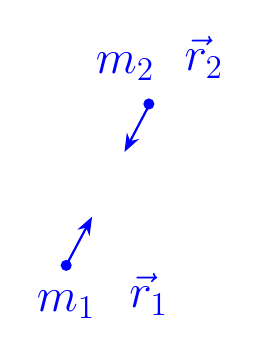
\begin{tikzpicture}[>=Stealth,thick,every node/.style={font=\fontsize{18}{22}\selectfont}]
  % dotted "graph paper" background


  % --- particle m1 and its position vector r1 ---
  \coordinate (M1) at (1.05,1.05);
  \fill[blue] (M1) circle (2pt);
  \draw[->,blue] (M1) -- ++(62.01:0.7);
  \node[blue] at (1.05,0.55) {$m_1$};
  \node[blue] at (2.1,0.68) {$\vec r_1$};

  % --- particle m2 and its position vector r2 ---
  \coordinate (M2) at (2.1,3.1);
  \fill[blue] (M2) circle (2pt);
  \node[blue] at (1.8,3.57) {$m_2$};
  \draw[->,blue] (2.1,3.08) -- (1.79,2.49);
  \node[blue] at (2.8,3.69) {$\vec r_2$};
\end{tikzpicture}
\end{document}
